\documentclass[12pt,a4paper,oneside]{article}

\usepackage[utf8]{inputenc}
\usepackage[portuguese]{babel}
\usepackage[T1]{fontenc}
\usepackage{amsmath}
\usepackage{amsfonts}
\usepackage{amssymb}
\usepackage{graphicx}
\usepackage{pgf}
\usepackage{tikz}
\usetikzlibrary{arrows,automata,positioning}

\usepackage{xcolor}
% Definindo novas cores
\definecolor{verde}{rgb}{0.25,0.5,0.35}
\definecolor{jpurple}{rgb}{0.5,0,0.35}
% Configurando layout para mostrar codigos Java
\usepackage{listings}
\lstset{
  language=Java,
  basicstyle=\ttfamily\small, 
  keywordstyle=\color{jpurple}\bfseries,
  stringstyle=\color{red},
  commentstyle=\color{verde},
  morecomment=[s][\color{blue}]{/**}{*/},
  extendedchars=true, 
  showspaces=false, 
  showstringspaces=false, 
  numbers=left,
  numberstyle=\tiny,
  breaklines=true, 
  backgroundcolor=\color{cyan!10}, 
  breakautoindent=true, 
  captionpos=b,
  xleftmargin=0pt,
  tabsize=4,
  escapeinside=||
}

\author{\\Universidade Federal de Goiás (UFG) - Câmpus Jataí\\Bacharelado em Ciência da Computação \\Inteligência Artificial \\Esdras Lins Bispo Jr.}

\title{\sc \huge Primeira Prova}

\begin{document}

\maketitle

{\bf ORIENTAÇÕES PARA A RESOLUÇÃO}

\begin{itemize}
	\item A avaliação é individual, sem consulta;
	\item A pontuação máxima desta avaliação é 10,0 (dez) pontos, sendo uma das 04 (quatro) componentes que formarão a média final da disciplina: duas provas, um projeto e exercícios;
	\item A média final será calculada pela média ponderada das quatro supraditas notas [em que a primeira prova tem peso 35 (trinta e cinco), a segunda prova tem peso 25 (vinte e cinco), o projeto tem peso 30 (trinta) e os exercícios-bônus são adicionados à media final];
	\item O somatório da pontuação de todas as questões desta avaliação é 11,0 (onze) pontos. Isto é um sinônimo de tolerância na correção. Se você por acaso perder 1,5 (um e meio), sua nota será 9,5 (nove e meio);
	\item O conteúdo exigido compreende os seguintes pontos apresentados no Plano de Ensino da disciplina: (1) Introdução à Inteligência Artificial, (2) Agentes Inteligentes, (3) Resolução de Problemas, (7) Aprendizado de Máquina e (8) Mineração de dados.
\end{itemize}

\begin{center}
	\fbox{\large Nome: \hspace{10cm}}
	\fbox{\large Assinatura: \hspace{9cm}}
\end{center}

\newpage

\begin{enumerate}

	\item (2,5 pt) ```Sem dúvida, os computadores não podem ser inteligentes - eles só podem fazer o que seus programadores determinam''. Esta última afirmação é verdadeira e implica a primeira? Justifique sua resposta baseado na discussão sobre as várias definições de Inteligência Artificial.
	
	{\color{blue} 
		{\bf Resposta:} A última afirmação é verdadeira: ``os computadores só podem fazer o que seus programadores determinam''. Mas não necessariamente implica a primeira. Isto acontece devido às várias concepções que podemos ter sobre o que é ser inteligente.
		
		Por exemplo, se a sua definição de inteligência for o grau de semelhança que o computador tem com a inteligência humana, temos pelo menos duas perspectivas a considerar. 
		
		A primeira perspectiva pode ser mais materialista, admitindo de certa forma que ``os seres humanos são máquinas determinadas pela sua matéria''. Nesta perspectiva, a última afirmação não implica a primeira.
		
		Porém, em uma segunda perspectiva não-materialista, pode-se admitir que ``os seres humanos são compostos por estruturas que vão além da matéria'' e, logo, não são necessariamente determinísticos. Assim, a última afirmação implica a primeira.
	}
	 	
	\item (2,5 pt) [ENADE 2008] A figura abaixo mostra uma árvore de decisão construída por um algoritmo de aprendizado indutivo a partir de um conjunto de dados em que os objetos são descritos por 4 atributos: $X1$, $X2$, $X3$ e $X4$. Dado um objeto de classe desconhecida, essa árvore classifica o objeto na classe 1 ou na classe 2. 

		\begin{center}
			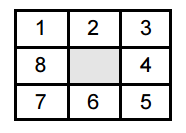
\includegraphics[width=8cm]{images/enade01.png}
		\end{center}
	
		A tabela a seguir apresenta três objetos a serem classificados: O1, O2 e O3.
		
		\begin{center}
			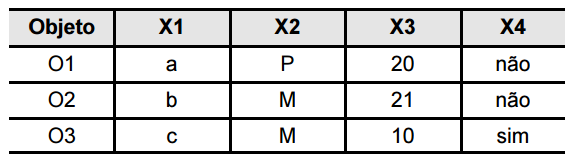
\includegraphics[width=8cm]{images/enade02.png}
		\end{center}
		
		A que classes corresponderiam, respectivamente, os objetos $O1$, $O2$ e $O3$? Assinale a opção correta abaixo {\bf e justifique a sua resposta}.
	
		\begin{enumerate}
			\item 1, 1 e 2
			\item 1, 2 e 1
			\item 2, 1 e 2
			\item 2, 2 e 1
			\item 1, 1 e 1
		\end{enumerate}	
	
	{ \color{blue}
		{\bf Resposta:} Basta navegarmos pela árvore decisão a partir dos atributos de cada objeto. Para o objeto O1, temos: 
		\begin{center}
			X1 $\xrightarrow{a}$ X3 $\xrightarrow{20}$ 1
		\end{center}
	Já para o objeto O2, temos: 
	\begin{center}
		X1 $\xrightarrow{b}$ 1
	\end{center}
 Por fim, para o objeto O3, temos: 
\begin{center}
	X1 $\xrightarrow{c}$ X2 $\xrightarrow{M}$ 2
\end{center}
Assim, a resposta correta é a letra (a).
	}

	\newpage
	
	\item (3,0 pt) Considere um espaço de estados em que o estado inicial é o número 1 e a função sucessor para o estado $n$ retorna dois estados, com números $2n$ e $2n+1$.

		\begin{enumerate}
			\item (1,0 pt) Desenhe a porção do espaço de estados correspondente aos estados de 1 a 15. \\
			
			{\color{blue} {\bf Resposta:}}
			
			\begin{tikzpicture}[->,>=stealth',shorten >=1pt,auto,node distance=1.5cm,
			semithick, draw=blue]
				\tikzstyle{every state}=
				[fill=blue,draw=none,text=white]
				
				\node[state] (O) 				{15};
				\node[state] (N) 	[left of=O] {14};
				\node[state] (M) 	[left of=N] {13};
				\node[state] (L) 	[left of=M] {12};
				\node[state] (K) 	[left of=L] {11};
				\node[state] (J) 	[left of=K] {10};
				\node[state] (I) 	[left of=J] {9};
				\node[state] (H) 	[left of=I] {8};
				
				\node[state] (G) 	[above left = 1cm and 0.3cm of O] {7};
				\node[state] (F) 	[above left = 1cm and 0.3cm of M] {6};
				\node[state] (E) 	[above left = 1cm and 0.3cm of K] {5};
				\node[state] (D) 	[above left = 1cm and 0.3cm of I] {4};
				
				\node[state] (C) 	[above left = 1cm and 1cm of G] {3};
				\node[state] (B) 	[above right = 1cm and 0.7cm of D] {2};
				
				\node[state] (A) 	[above left = 1cm and 2.2cm of C] {1};
				
				\path 	(A) edge node {} (B)
						(A) edge node {} (C)
						(B) edge node {} (D)
						(B) edge node {} (E)
						(C) edge node {} (F)
						(C) edge node {} (G)
						(D) edge node {} (H)
						(D) edge node {} (I)
						(E) edge node {} (J)
						(E) edge node {} (K)
						(F) edge node {} (L)
						(F) edge node {} (M)
						(G) edge node {} (N)
						(G) edge node {} (O);
			\end{tikzpicture}
			
			\hspace*{1cm}
			
			\item (1,5 pt) Suponha que o estado objetivo seja 11. Admitindo apenas a porção feita na letra (a), liste a ordem em que os nós serão visitados no caso da busca em extensão (largura) e a busca em profundidade.\\
			
			{\color{blue} 
				{\bf Resposta:} Ordem de visitação da busca em extensão:
				\begin{center}
					1, 2, 3, 4, 5, 6, 7, 8, 9, 10 e 11.
				\end{center}
				Ordem de visitação da busca em profundidade:
				\begin{center}
					1, 2, 4, 8, 9, 5, 10 e 11.
				\end{center}
			}
		\end{enumerate}
	
	\newpage
	
	\item (3,0 pt) Construa o índice invertido (conforme apresentado em sala de aula) para a coleção de documentos abaixo:
		
		\begin{itemize}
			\item[] {\bf Doc1} \ \ breakthrough drug for schizophrenia
			\item[] {\bf Doc2} \ \ new schizophrenia drug
			\item[] {\bf Doc3} \ \ new approach for treatment of schizophrenia
			\item[] {\bf Doc4} \ \ new hopes for schizophrenia patients
		\end{itemize}
	
	{\color{blue} 
		{\bf Resposta:} \underline{Passo 1} - Tokenização\\
		\begin{center}
			\begin{tabular}{cc}
				\hline
				Termos			&	DocID	\\
				\hline	
				breakthrough	&	1		\\
				drug			&	1		\\
				for				&	1		\\
				schizophrenia	&	1		\\
				new				&	2		\\
				schizophrenia	&	2		\\
				drug			&	2		\\
				new				&	3		\\ 
				approach		&	3		\\ 
				for 			&	3		\\
				treatment 		&	3		\\
				of 				&	3		\\
				schizophrenia	&	3		\\
				new 			&	4		\\
				hopes 			&	4		\\
				for 			&	4		\\
				schizophrenia 	&	4		\\
				patients		&	4		\\
				\hline			
			\end{tabular}
		\end{center}
	
	\newpage
	\underline{Passo 2} - Ordem Alfabética\\
	
		\begin{center}
			\begin{tabular}{cc}
				\hline
				Termos			&	DocID	\\
				\hline	
				approach		&	3		\\ 
				breakthrough	&	1		\\
				drug			&	1		\\
				drug			&	2		\\
				for				&	1		\\
				for 			&	3		\\
				for 			&	4		\\
				hopes 			&	4		\\
				new				&	2		\\
				new				&	3		\\ 
				new 			&	4		\\
				of 				&	3		\\
				patients		&	4		\\
				schizophrenia	&	1		\\
				schizophrenia	&	2		\\
				schizophrenia	&	3		\\
				schizophrenia 	&	4		\\
				treatment 		&	3		\\
				\hline			
			\end{tabular}
		\end{center}
	
		\underline{Passo 3} - Agrupamento\\
	
		\begin{center}
			\begin{tabular}{rl}
				\hline
				Termo / Freq. Doc.	&	Lista de {\it Postings}	 \\
				\hline	
				\fbox{approach | 1}		&	$\fbox{3}$	\\ 
				\fbox{breakthrough | 1}	&	$\fbox{3}$ \\ 
				\fbox{drug | 2}			&	
				$\fbox{1} \rightarrow \fbox{2}$ \\ 
				\fbox{for | 3}				&	
				$\fbox{1} \rightarrow \fbox{3} \rightarrow \fbox{4}$ \\
				\fbox{hopes | 1} 			&	$\fbox{4}$ \\ 
				\fbox{new | 3}				&
				$\fbox{2} \rightarrow \fbox{3} \rightarrow \fbox{4}$ \\
				\fbox{of | 1} 				&	$\fbox{3}$ \\ 
				\fbox{patients | 1}		&	$\fbox{4}$ \\ 
				\fbox{schizophrenia | 4}	&	
				$\fbox{1} \rightarrow \fbox{2} \rightarrow \fbox{3} \rightarrow \fbox{4}$ \\ 
				\fbox{treatment | 1}		&	$\fbox{3}$ \\  
				\hline			
			\end{tabular}
		\end{center}	
	
	}
	
	\end{enumerate}
\end{document}